\documentclass[__main__.tex]{subfiles}

\begin{document}

\qtitle{П}{10}
Воспользуйтесь связью полей $\vec{E}$ и $\vec{B}$ с 4-векторным потенциалом $A^\mu$, чтобы отождествить $(0,j)$-ю компоненту симметризованного тензора энергии-импульса электромагнитного поля с $j$-й компонентой вектора Пойнтинга: $\Theta^{0j}=\left(\vec{E}\times\vec{B}\right)^{j}$. Запишите и прокомментируйте теорему Пойнтинга для свободного электромагнитного поля.\\ 

Воспользуемся выведенным на лекции представлением тензора энергии-импульса ЭМП:
\begin{gather*}
	\Theta^{\mu\nu} = F\indices{^\mu_\rho}F^{\nu\rho}-\frac{1}{4}\eta^{\mu\nu}F_{\alpha\beta}F^{\alpha\beta},\\
	\eta^{\mu\nu}=diag(-1,1,1,1)\;остальные\;элементы\;0.
\end{gather*}
Дальше будет приведено изображение тензора Максвелла с разными индексами. Те элементы, которые должны стоять в решетке совпадают с элементами тензора с нижними индексами. Напоминаю, что индексация у Ники идёт с нуля а не с единицы.
\begin{figure}[h]
\center{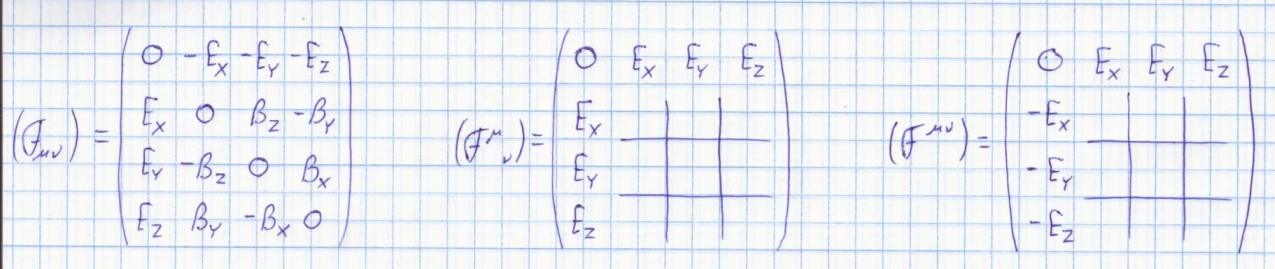
\includegraphics[width=\linewidth]{P-10}}
\end{figure}

Нам нужно получить (0;j) компоненту, где j=1,2,3 . Легко заметить, что матрица $\eta$ имеет нули в этих местах, поэтому работаем только с уменьшаемым:
\begin{gather*}
	\Theta^{01} = F\indices{^0_i}F^{1i} = E_yB_z-E_zB_y\\
	\Theta^{02} = F\indices{^0_i}F^{2i} = -E_xB_z+E_zB_x\\
	\Theta^{03} = F\indices{^0_i}F^{3i} = E_xB_y-E_yB_x\Rightarrow\\
	\Theta^{0j}=\left(\vec{E}\times\vec{B}\right)^{j}
\end{gather*}

\begin{theorem}
	$\frac{\partial U}{\partial t}+\nabla\cdot S = -J\cdot E$\;,\; где $U = \frac{E\cdot D}{2}+\frac{B\cdot H}{2}$ - плотность энергии ЭМП ( (0;0) компонента тензора энергии-импульса ), $S=\left[E\times B\right]$ - вектор Пойнтинга, $J=\sigma E$ - плотность тока, D - электрическая индукция (пропорциональна Е), H - напряженность МП (пропорциональна В)
\end{theorem}
Смысл этой теоремы в следующем: скорость возрастания электромагнитной энергии внутри некоторого объема в сумме с энергией, вытекающей за единицу времени через поверхность, ограничивающую этот объем, равна с минусом полной работе, совершаемой полем над источниками внутри данного объема.
\end{document}